\documentclass[]{article}
\usepackage{lmodern}
\usepackage{amssymb,amsmath}
\usepackage{ifxetex,ifluatex}
\usepackage{fixltx2e} % provides \textsubscript
\ifnum 0\ifxetex 1\fi\ifluatex 1\fi=0 % if pdftex
  \usepackage[T1]{fontenc}
  \usepackage[utf8]{inputenc}
\else % if luatex or xelatex
  \ifxetex
    \usepackage{mathspec}
  \else
    \usepackage{fontspec}
  \fi
  \defaultfontfeatures{Ligatures=TeX,Scale=MatchLowercase}
\fi
% use upquote if available, for straight quotes in verbatim environments
\IfFileExists{upquote.sty}{\usepackage{upquote}}{}
% use microtype if available
\IfFileExists{microtype.sty}{%
\usepackage{microtype}
\UseMicrotypeSet[protrusion]{basicmath} % disable protrusion for tt fonts
}{}
\usepackage[margin=1in]{geometry}
\usepackage{hyperref}
\hypersetup{unicode=true,
            pdftitle={SELECTED pieces form: Contrasting TLS-derived orthogonal stem profiles, in poplar plantations},
            pdfauthor={Puletti N., Grotti M., Scotti R.},
            pdfborder={0 0 0},
            breaklinks=true}
\urlstyle{same}  % don't use monospace font for urls
\usepackage{color}
\usepackage{fancyvrb}
\newcommand{\VerbBar}{|}
\newcommand{\VERB}{\Verb[commandchars=\\\{\}]}
\DefineVerbatimEnvironment{Highlighting}{Verbatim}{commandchars=\\\{\}}
% Add ',fontsize=\small' for more characters per line
\usepackage{framed}
\definecolor{shadecolor}{RGB}{248,248,248}
\newenvironment{Shaded}{\begin{snugshade}}{\end{snugshade}}
\newcommand{\AlertTok}[1]{\textcolor[rgb]{0.94,0.16,0.16}{#1}}
\newcommand{\AnnotationTok}[1]{\textcolor[rgb]{0.56,0.35,0.01}{\textbf{\textit{#1}}}}
\newcommand{\AttributeTok}[1]{\textcolor[rgb]{0.77,0.63,0.00}{#1}}
\newcommand{\BaseNTok}[1]{\textcolor[rgb]{0.00,0.00,0.81}{#1}}
\newcommand{\BuiltInTok}[1]{#1}
\newcommand{\CharTok}[1]{\textcolor[rgb]{0.31,0.60,0.02}{#1}}
\newcommand{\CommentTok}[1]{\textcolor[rgb]{0.56,0.35,0.01}{\textit{#1}}}
\newcommand{\CommentVarTok}[1]{\textcolor[rgb]{0.56,0.35,0.01}{\textbf{\textit{#1}}}}
\newcommand{\ConstantTok}[1]{\textcolor[rgb]{0.00,0.00,0.00}{#1}}
\newcommand{\ControlFlowTok}[1]{\textcolor[rgb]{0.13,0.29,0.53}{\textbf{#1}}}
\newcommand{\DataTypeTok}[1]{\textcolor[rgb]{0.13,0.29,0.53}{#1}}
\newcommand{\DecValTok}[1]{\textcolor[rgb]{0.00,0.00,0.81}{#1}}
\newcommand{\DocumentationTok}[1]{\textcolor[rgb]{0.56,0.35,0.01}{\textbf{\textit{#1}}}}
\newcommand{\ErrorTok}[1]{\textcolor[rgb]{0.64,0.00,0.00}{\textbf{#1}}}
\newcommand{\ExtensionTok}[1]{#1}
\newcommand{\FloatTok}[1]{\textcolor[rgb]{0.00,0.00,0.81}{#1}}
\newcommand{\FunctionTok}[1]{\textcolor[rgb]{0.00,0.00,0.00}{#1}}
\newcommand{\ImportTok}[1]{#1}
\newcommand{\InformationTok}[1]{\textcolor[rgb]{0.56,0.35,0.01}{\textbf{\textit{#1}}}}
\newcommand{\KeywordTok}[1]{\textcolor[rgb]{0.13,0.29,0.53}{\textbf{#1}}}
\newcommand{\NormalTok}[1]{#1}
\newcommand{\OperatorTok}[1]{\textcolor[rgb]{0.81,0.36,0.00}{\textbf{#1}}}
\newcommand{\OtherTok}[1]{\textcolor[rgb]{0.56,0.35,0.01}{#1}}
\newcommand{\PreprocessorTok}[1]{\textcolor[rgb]{0.56,0.35,0.01}{\textit{#1}}}
\newcommand{\RegionMarkerTok}[1]{#1}
\newcommand{\SpecialCharTok}[1]{\textcolor[rgb]{0.00,0.00,0.00}{#1}}
\newcommand{\SpecialStringTok}[1]{\textcolor[rgb]{0.31,0.60,0.02}{#1}}
\newcommand{\StringTok}[1]{\textcolor[rgb]{0.31,0.60,0.02}{#1}}
\newcommand{\VariableTok}[1]{\textcolor[rgb]{0.00,0.00,0.00}{#1}}
\newcommand{\VerbatimStringTok}[1]{\textcolor[rgb]{0.31,0.60,0.02}{#1}}
\newcommand{\WarningTok}[1]{\textcolor[rgb]{0.56,0.35,0.01}{\textbf{\textit{#1}}}}
\usepackage{graphicx,grffile}
\makeatletter
\def\maxwidth{\ifdim\Gin@nat@width>\linewidth\linewidth\else\Gin@nat@width\fi}
\def\maxheight{\ifdim\Gin@nat@height>\textheight\textheight\else\Gin@nat@height\fi}
\makeatother
% Scale images if necessary, so that they will not overflow the page
% margins by default, and it is still possible to overwrite the defaults
% using explicit options in \includegraphics[width, height, ...]{}
\setkeys{Gin}{width=\maxwidth,height=\maxheight,keepaspectratio}
\IfFileExists{parskip.sty}{%
\usepackage{parskip}
}{% else
\setlength{\parindent}{0pt}
\setlength{\parskip}{6pt plus 2pt minus 1pt}
}
\setlength{\emergencystretch}{3em}  % prevent overfull lines
\providecommand{\tightlist}{%
  \setlength{\itemsep}{0pt}\setlength{\parskip}{0pt}}
\setcounter{secnumdepth}{0}
% Redefines (sub)paragraphs to behave more like sections
\ifx\paragraph\undefined\else
\let\oldparagraph\paragraph
\renewcommand{\paragraph}[1]{\oldparagraph{#1}\mbox{}}
\fi
\ifx\subparagraph\undefined\else
\let\oldsubparagraph\subparagraph
\renewcommand{\subparagraph}[1]{\oldsubparagraph{#1}\mbox{}}
\fi

%%% Use protect on footnotes to avoid problems with footnotes in titles
\let\rmarkdownfootnote\footnote%
\def\footnote{\protect\rmarkdownfootnote}

%%% Change title format to be more compact
\usepackage{titling}

% Create subtitle command for use in maketitle
\newcommand{\subtitle}[1]{
  \posttitle{
    \begin{center}\large#1\end{center}
    }
}

\setlength{\droptitle}{-2em}

  \title{SELECTED pieces form: Contrasting TLS-derived orthogonal stem profiles,
in poplar plantations}
    \pretitle{\vspace{\droptitle}\centering\huge}
  \posttitle{\par}
    \author{Puletti N., Grotti M., Scotti R.}
    \preauthor{\centering\large\emph}
  \postauthor{\par}
      \predate{\centering\large\emph}
  \postdate{\par}
    \date{september 2018}


\begin{document}
\maketitle

{
\setcounter{tocdepth}{2}
\tableofcontents
}
\hypertarget{plot-selected-profiles}{%
\section{Plot selected profiles}\label{plot-selected-profiles}}

\begin{verbatim}
## # A tibble: 12 x 3
##    Treat treid treid2
##    <chr> <chr> <chr> 
##  1 V400  s01   A     
##  2 V400  s03   B     
##  3 V400  s07   C     
##  4 V400  s12   D     
##  5 V450  s07   A     
##  6 V450  s08   B     
##  7 V450  s09   C     
##  8 V450  s12   D     
##  9 V500  s03   A     
## 10 V500  s04   B     
## 11 V500  s08   C     
## 12 V500  s12   D
\end{verbatim}

\begin{verbatim}
## Joining, by = c("Treat", "treid")
\end{verbatim}

\begin{verbatim}
## Warning: Column `Treat` joining factor and character vector, coercing into
## character vector
\end{verbatim}

\begin{verbatim}
## Warning: Column `treid` joining factor and character vector, coercing into
## character vector
\end{verbatim}

\includegraphics{AnalysisOfTLSbasedOrthogonalStemProfiles_SelectedOutputs_files/figure-latex/plot1-1.svg}

\begin{verbatim}
## Saving 3.2 x 5 in image
\end{verbatim}

\hypertarget{quantitative-effects}{%
\section{Quantitative effects}\label{quantitative-effects}}

\begin{Shaded}
\begin{Highlighting}[]
\KeywordTok{library}\NormalTok{(kableExtra)}

\NormalTok{TLSdbh_df <-}\StringTok{ }\NormalTok{tff }\OperatorTok\StringTok{ }
\StringTok{  }\KeywordTok{filter}\NormalTok{(}\KeywordTok{abs}\NormalTok{(}\FloatTok{1.3} \OperatorTok{-}\StringTok{ }\NormalTok{Sect_height)}\OperatorTok{<}\NormalTok{.}\DecValTok{0001}\NormalTok{) }\OperatorTok\StringTok{ }
\StringTok{  }\KeywordTok{select}\NormalTok{(Treat, treid, TreeId, }\DataTypeTok{dbh =}\NormalTok{ DBH, }\KeywordTok{starts_with}\NormalTok{(}\StringTok{'diam'}\NormalTok{)) }\OperatorTok
\StringTok{  }\KeywordTok{gather}\NormalTok{(direction, TLSdbh, }\KeywordTok{starts_with}\NormalTok{(}\StringTok{'diam'}\NormalTok{)) }\OperatorTok
\StringTok{  }\KeywordTok{mutate}\NormalTok{(}\DataTypeTok{TLSdbh =} \DecValTok{100} \OperatorTok{*}\StringTok{ }\NormalTok{TLSdbh) }

\NormalTok{TLSdbh_df }\OperatorTok
\StringTok{  }\KeywordTok{lm}\NormalTok{(TLSdbh }\OperatorTok{~}\StringTok{ }\NormalTok{Treat }\OperatorTok{+}\StringTok{ }\NormalTok{direction, }\DataTypeTok{data =}\NormalTok{ .) }\OperatorTok
\StringTok{  }\KeywordTok{summary}\NormalTok{() }\OperatorTok\StringTok{ }\KeywordTok{tidy}\NormalTok{() }\OperatorTok
\StringTok{  }\KeywordTok{kable}\NormalTok{(}\DataTypeTok{digits =}\KeywordTok{c}\NormalTok{(}\DecValTok{0}\NormalTok{, }\DecValTok{2}\NormalTok{, }\DecValTok{3}\NormalTok{, }\DecValTok{3}\NormalTok{, }\DecValTok{5}\NormalTok{), }\DataTypeTok{format =} \StringTok{"latex"}\NormalTok{,}
        \DataTypeTok{caption =} \StringTok{"Sideways compression of dbh and plantation density effects"}\NormalTok{)}
\end{Highlighting}
\end{Shaded}

\begin{table}

\caption{\label{tab:unnamed-chunk-1}Sideways compression of dbh and plantation density effects}
\centering
\begin{tabular}[t]{l|r|r|r|r}
\hline
term & estimate & std.error & statistic & p.value\\
\hline
(Intercept) & 37.54 & 0.540 & 69.560 & 0.00000\\
\hline
TreatV450 & 2.09 & 0.661 & 3.158 & 0.00237\\
\hline
TreatV500 & 2.60 & 0.661 & 3.928 & 0.00020\\
\hline
directiondiam\_wti\_rows & -1.84 & 0.540 & -3.401 & 0.00113\\
\hline
\end{tabular}
\end{table}

\hypertarget{grafico-conclusivo}{%
\section{Grafico conclusivo}\label{grafico-conclusivo}}

\begin{Shaded}
\begin{Highlighting}[]
\NormalTok{tff }\OperatorTok\StringTok{ }
\StringTok{  }\KeywordTok{filter}\NormalTok{(Segm_length }\OperatorTok{==}\StringTok{ }\FloatTok{0.1}\NormalTok{) }\OperatorTok
\StringTok{  }\KeywordTok{group_by}\NormalTok{(Sect_height, Treat) }\OperatorTok
\StringTok{  }\KeywordTok{summarise}\NormalTok{(}\DataTypeTok{mean_delta =} \KeywordTok{mean}\NormalTok{(delta_d_cm)) }\OperatorTok
\StringTok{  }\KeywordTok{mutate}\NormalTok{(}\DataTypeTok{Treat =} \KeywordTok{recode_factor}\NormalTok{(Treat, }
                  \DataTypeTok{V400 =} \StringTok{"4.0"}\NormalTok{, }\DataTypeTok{V450 =} \StringTok{"4.5"}\NormalTok{, }\DataTypeTok{V500 =} \StringTok{"5.0"}\NormalTok{)) }\OperatorTok
\StringTok{  }\KeywordTok{ggplot}\NormalTok{(}\KeywordTok{aes}\NormalTok{(}\DataTypeTok{x =}\NormalTok{ Sect_height, }\DataTypeTok{y =}\NormalTok{ mean_delta, }\DataTypeTok{linetype =}\NormalTok{ Treat)) }\OperatorTok{+}
\StringTok{  }\KeywordTok{geom_smooth}\NormalTok{(}\DataTypeTok{colour =} \StringTok{"grey40"}\NormalTok{) }\OperatorTok{+}
\StringTok{  }\KeywordTok{theme_bw}\NormalTok{() }\OperatorTok{+}
\StringTok{  }\KeywordTok{theme}\NormalTok{(}\DataTypeTok{legend.position =} \KeywordTok{c}\NormalTok{(}\FloatTok{0.8}\NormalTok{, }\FloatTok{0.7}\NormalTok{),}
        \DataTypeTok{legend.background =} 
          \KeywordTok{element_rect}\NormalTok{(}\DataTypeTok{size=}\FloatTok{0.5}\NormalTok{, }\DataTypeTok{linetype=}\StringTok{"solid"}\NormalTok{, }\DataTypeTok{colour =}\StringTok{"grey"}\NormalTok{)) }\OperatorTok{+}
\StringTok{  }\KeywordTok{guides}\NormalTok{(}\DataTypeTok{linetype =} \KeywordTok{guide_legend}\NormalTok{(}\DataTypeTok{title=}
        \StringTok{"distance [m]}\CharTok{\textbackslash{}n}\StringTok{to nearest}\CharTok{\textbackslash{}n}\StringTok{competitor"}\NormalTok{)) }\OperatorTok{+}
\StringTok{  }\KeywordTok{ylab}\NormalTok{(}\StringTok{"diameter difference [cm]"}\NormalTok{) }\OperatorTok{+}
\StringTok{  }\KeywordTok{xlab}\NormalTok{(}\StringTok{"height of the section [m]"}\NormalTok{) }\OperatorTok{+}
\StringTok{  }\KeywordTok{ggtitle}\NormalTok{(}\StringTok{"Compression of the stems horizontal crosssections"}\NormalTok{, }
          \DataTypeTok{subtitle =} \StringTok{"difference between the diameter along the low-competitiondirection and that along the high-competition-direction"}\NormalTok{)}
\end{Highlighting}
\end{Shaded}

\begin{verbatim}
## `geom_smooth()` using method = 'loess' and formula 'y ~ x'
\end{verbatim}

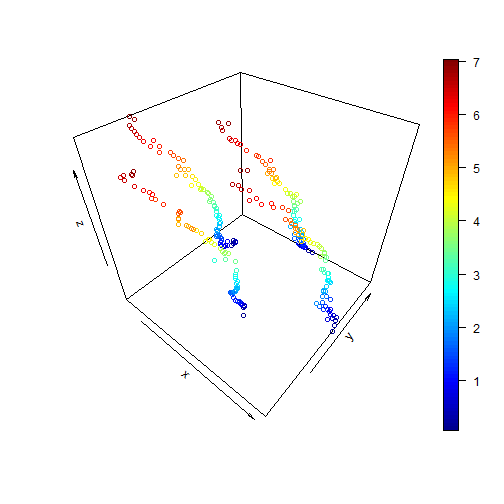
\includegraphics{AnalysisOfTLSbasedOrthogonalStemProfiles_SelectedOutputs_files/figure-latex/unnamed-chunk-2-1.pdf}


\end{document}
